\documentclass[a4]{article}
\usepackage{geometry}
\geometry{verbose,tmargin=2.5cm,bmargin=2.5cm,lmargin=3cm,rmargin=3cm}
\usepackage{amsmath,amssymb,amsthm}
\usepackage{graphicx}
\graphicspath{{graphics/}}
\usepackage[utf8]{inputenc}
\usepackage{fancyvrb}
\usepackage{hyperref}
\usepackage{lscape}
\usepackage{adjustbox}
\usepackage{verbatim}
\usepackage{subcaption}
\usepackage{placeins}


\title{MultiFEBE \\ ME-TH-AC-001 [TUTORIAL] \\ Pressure waves in a room (BEM model)}

\author{J.D.R. Bordón}

\date{September 2024}

\begin{document}

\maketitle

\tableofcontents 

\section{Problem description}

In this tutorial, the acoustic response of a room with a given set of boundary conditions is obtained. Figure \ref{fig:problem} shows the room with the most relevant data. 

\begin{figure}[h]
\centering
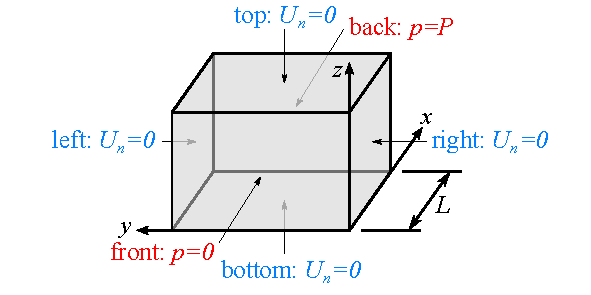
\includegraphics[scale=1]{problem.pdf}
\caption{Problem layout\label{fig:problem}}
\end{figure}

It is a cubic room with side length $L$. Bottom, top, left and right walls are rigid walls, and thus there is no fluid displacement in the normal direction of these walls ($U_n=0\,\mathrm{m}$). Front and back walls have prescribed dynamic pressures, being null on the front wall ($p(x=0)=0\,\mathrm{Pa}$) and a given value $P=1\,\mathrm{Pa}$ on the back wall ($p(x=L)=1\,\mathrm{Pa}$). Therefore, the solution is one-dimensional and the analytical solution can be easily obtained.
 
The domain $\Omega$ (air inside the room) contain an inviscid fluid with density $\rho=1.25\,\mathrm{kg/m^3}$, and the wave propagation speed (speed of sound) is $c=343\,\mathrm{m/s}$. The basic acoustic phenomena is governed by the Helmholtz differential equation (scalar wave propagation), see e.g. \cite{dominguez,maeso}. For this problem, the solution consists of two plane waves travelling in opposite directions along $x$:
\begin{equation}
p=p\left(x\right) = A\mathrm{e}^{-ikx} + B\mathrm{e}^{ikx}
\end{equation}
where $A$ and $B$ are the amplitudes of the waves, $k=\omega/c$ is the wavenumber and $\omega$ is the circular frequency ($\omega=2\pi f$). Once boundary conditions are considered, the pressure $p$ and fluid displacement in the $x$ direction can be written as:
\begin{align}
p\left(x\right)   &= \frac{P}{\sin kL}\sin kx \\
U_x\left(x\right) &= \frac{1}{\rho\omega^2}\frac{\mathrm{d}\,p}{\mathrm{d}x} = \frac{Pk}{\rho\omega^2\sin kL}\cos kx
\end{align}
where natural frequencies are found when $\sin(kL)=0$, which occurs at:
\begin{equation}
f_n = \frac{n \pi c}{2 \pi L}
\end{equation}
with $n=1,\,2,...$, leading in this case to $f_1=57.167,\mathrm{Hz}$, $f_2=114.333,\mathrm{Hz}$, ...

\section{Pre-processing}

Many different BEM models could be considered for this problem with a one-dimensional response. In this tutorial, a fully three-dimensional BEM model is used. In the present model, the response along the walls are obtained through the discretization of the boundary into boundary elements. The solution within the domain is also obtained by using another type of entity called internal points (in the BEM, this is a post-processing stage).

\subsection{Geometry (*.geo file)}

Gmsh \cite{gmshweb} is used for defining the geometry and meshing it. Figure \ref{fig:geometry_partition} shows the geometry that is has been defined (see Gmsh file \texttt{./case\_files/cube.geo} with plain text editor and open it with Gmsh).  At the beginning of the file, appropriate variables are defined, in particular the side length of the cube ($L=3\,\mathrm{m}$), and the desired mesh element size. Then a set of points, lines, line loops and surfaces are defined. The boundary is partitioned into 6 surfaces, each one corresponding to each wall. Note that, unlike the FEM, the BEM discretization is not that intuitive, and some precautions must be taken into account.

On one hand, it is important to define each surface (and each boundary element) with the appropriate orientation. Given that the domain is defined by its boundary, each boundary piece must have the same orientation, otherwise the boundary of the domain is not compatible and the domain is undefined. By convention, the domain is defined by a boundary with outward normal. Figure \ref{fig:geometry_partition} shows the unit normals pointing outward the room, meaning that the modeled domain is the interior of the room. If the normals were pointing inwards, then the modeled domain is the exterior of the room.

On the other hand, there are some issues with the BEM which requires an appropriate discretization restrictions. One of the issues is the ``corner problem'' (a classic BEM issue, see e.g. \cite{brebbia}), and another is the appropriate representation of the stresses at corners and along edges. There are several approaches to solve these. One approach is the use of discontinuous elements, which automatically removes them, although at the same time it introduces primary variables discontinuities along the element edges (pressure in this case). Another approach is the use of special elements along these corners and edges. MultiFEBE uses a hybrid approach which consists on using continuous elements (conventional Lagrange elements with nodes at the element boundary), doubling the nodes where necessary, and  systematically performing a multiple non-nodal collocation at the boundary of each boundary element mesh. In essence, this approach is similar to the use of discontinuous elements at the boundary of each boundary element mesh, and thus leading to possible primary variables discontinuities only there.

From the user perspective, this means that the boundary of the domain must be completely divided (disconnected) along edges between parts of the boundary with different boundary conditions or sharp edges/corners. This means that along these edges nodes share their position but not connectivity. It is helpful to think that the boundary of the domain is divided by boundary partitions like a puzzle is divided by puzzle pieces. In other words, in the resulting geometry each boundary partition must have unique points and edges not shared by other boundary partitions.

\begin{figure}
  \centering
  \begin{subfigure}[b]{0.48\textwidth}
    \centering
    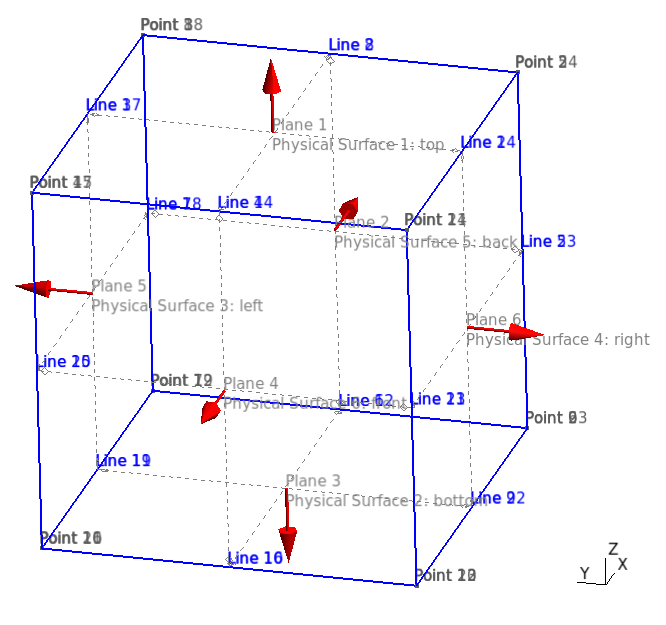
\includegraphics[width=\textwidth]{geometry_all.png}
    \caption{All wall}
    \label{fig:g1}
  \end{subfigure}
  \\
  \begin{subfigure}[b]{0.48\textwidth}
    \centering
    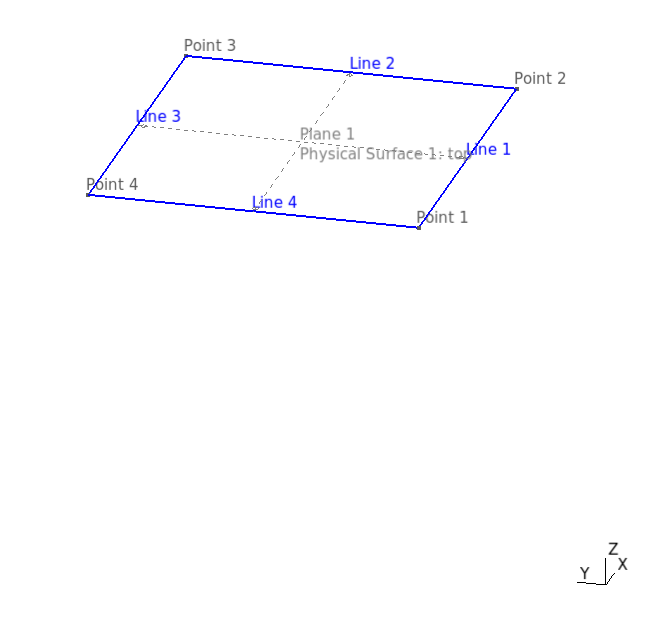
\includegraphics[width=\textwidth]{geometry_1.png}
    \caption{Top wall}
    \label{fig:g3}
  \end{subfigure}
  \begin{subfigure}[b]{0.48\textwidth}
    \centering
    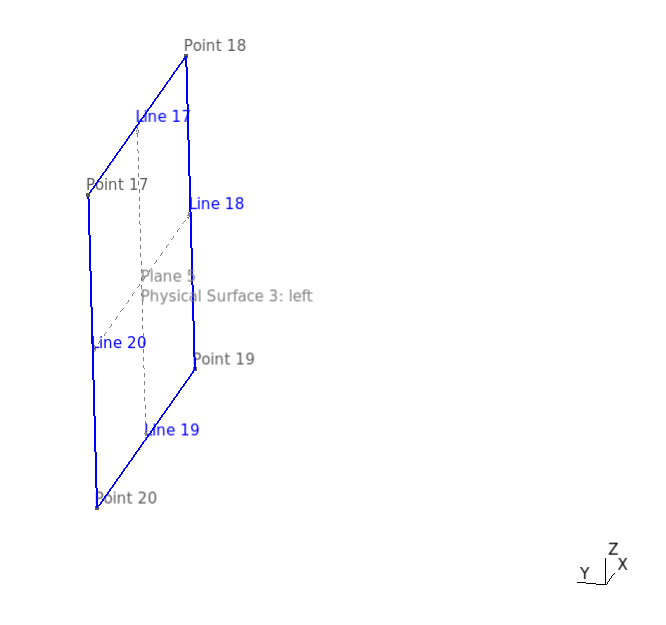
\includegraphics[width=\textwidth]{geometry_3.png}
    \caption{Left wall}
    \label{fig:g5}
  \end{subfigure}
  \hfill
  \begin{subfigure}[b]{0.48\textwidth}
    \centering
    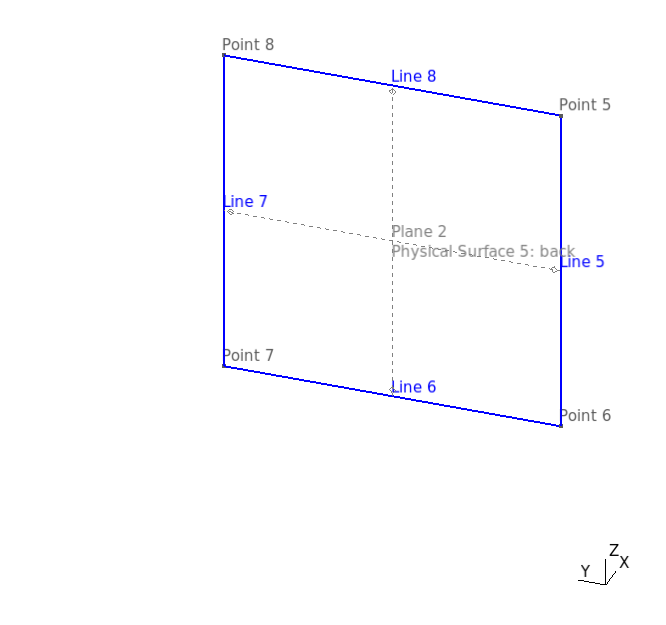
\includegraphics[width=\textwidth]{geometry_5.png}
    \caption{Back wall}
    \label{fig:g3}
  \end{subfigure}
  \hfill
  \begin{subfigure}[b]{0.48\textwidth}
    \centering
    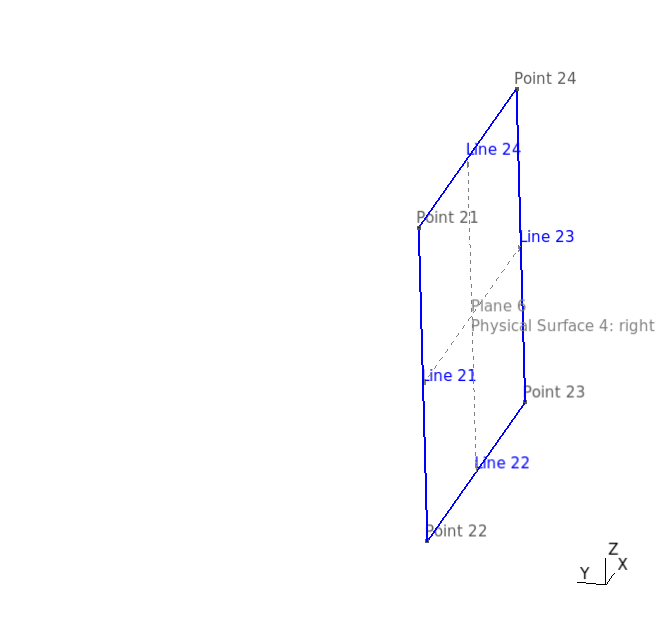
\includegraphics[width=\textwidth]{geometry_4.png}
    \caption{Right wall}
    \label{fig:g5}
  \end{subfigure}  
  \caption{Geometry. Note that along the geometry edges, lines and points are different for each wall.}
  \label{fig:geometry_partition}
\end{figure}

\subsection{Mesh (*.msh file)}

The mesh is generated by Gmsh from the Gmsh geometry file defined above (\texttt{./case\_files/cube.geo}). At the beginning of the \texttt{*.geo} file, the required mesh element size has been defined as:
\begin{Verbatim}[frame=single, fontsize=\small, label=cube.geo]
...

es = L/8; // Element size

...
\end{Verbatim}
At the end of this file, you will find the following lines:
\begin{Verbatim}[frame=single, fontsize=\small, label=cube.geo]
...

// Mesh of quadrilaterals. Comment the following lines to generate triangles
Transfinite Surface{1,2,3,4,5,6};
Recombine Surface {1,2,3,4,5,6};

// Mesh generation
Mesh 2;          // Generate up to surface elements
SetOrder 2;      // 1: linear, 2: quadratic
Save "cube.msh";
\end{Verbatim}
The first two lines allow the generation of a mesh of quadrilaterals (by default, it generates triangles). The next three lines are related to the mesh generation process: maximum dimension of elements to generate, element order and save the mesh in Gmsh format the name of the mesh file.

It is important to note that only Gmsh mesh file version 2.2 is allowed by MultiFEBE. From the command line, it can be generated as:
\begin{Verbatim}[frame=single, fontsize=\small, label=command line]
$ gmsh -2 -order 2 -format msh22 cube.msh
\end{Verbatim}
You can also generate it by running the Gmsh GUI (see the manual for more details). At the beginning of the \texttt{*.msh} file, you can check the Gmsh mesh format version, it must read as (remember, only version 2.2 can be read by MultiFEBE):
\begin{Verbatim}[frame=single, fontsize=\small, label=cube.geo]
$MeshFormat
2.2 0 8
$EndMeshFormat
\end{Verbatim}
Next, the list of physical entities (Gmsh jargon) are defined (Physical Lines, Physical Surfaces, ...) as defined in the *.geo file. 
\begin{Verbatim}[frame=single, fontsize=\small, label=cube.geo]
$PhysicalNames
6
2 1 "top"
2 2 "bottom"
2 3 "left"
2 4 "right"
2 5 "back"
2 6 "front"
$EndPhysicalNames
\end{Verbatim}
The first number is the number of physical entities. Then, each line defines each physical entity, where the first number can be: 0 (Physical Point), 1 (Physical Line), 2 (Physical Surface) and 3 (Physical Volume); the second number is the identifier/label of the physical entity, and last the name of the phyical entity. It is important to check the physical entity identifier (and the physical entity name), because these identifiers are later used.

In order to check the mesh, we will show the mesh but changing the element size to $L/2$ for the sake of clarity. Note that given that edges and points are not shared by the different boundary partitions (each wall), the produced nodes are not shared by different boundary partitions, i.e. each boundary partition has unique nodes.

\begin{figure}
  \centering
  \begin{subfigure}[b]{0.48\textwidth}
    \centering
    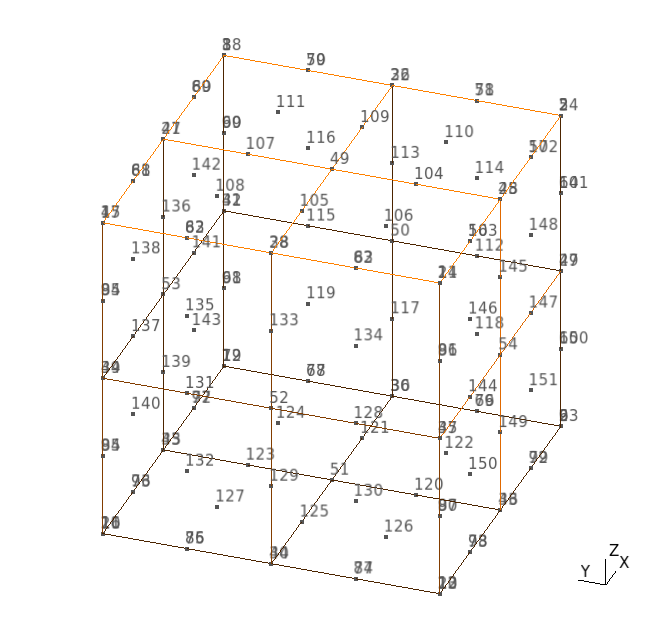
\includegraphics[width=\textwidth]{mesh_all.png}
    \caption{All wall}
    \label{fig:g1}
  \end{subfigure}
  \\
  \begin{subfigure}[b]{0.48\textwidth}
    \centering
    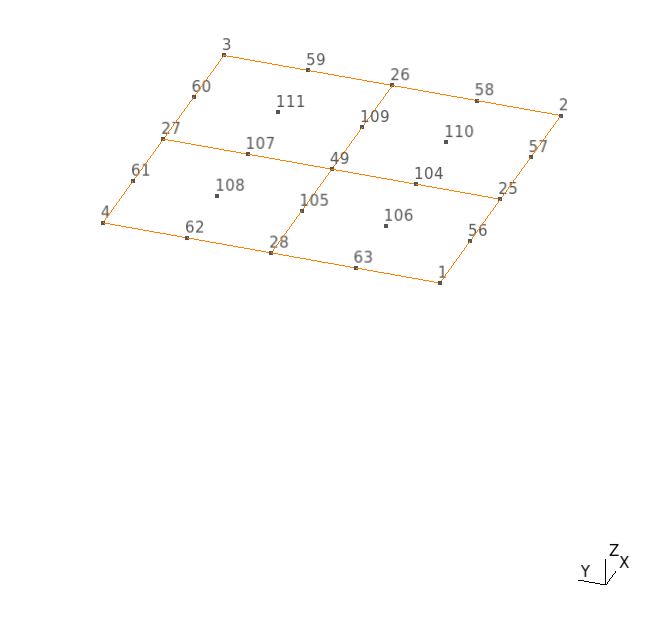
\includegraphics[width=\textwidth]{mesh_1.png}
    \caption{Top wall}
    \label{fig:g3}
  \end{subfigure}
  \begin{subfigure}[b]{0.48\textwidth}
    \centering
    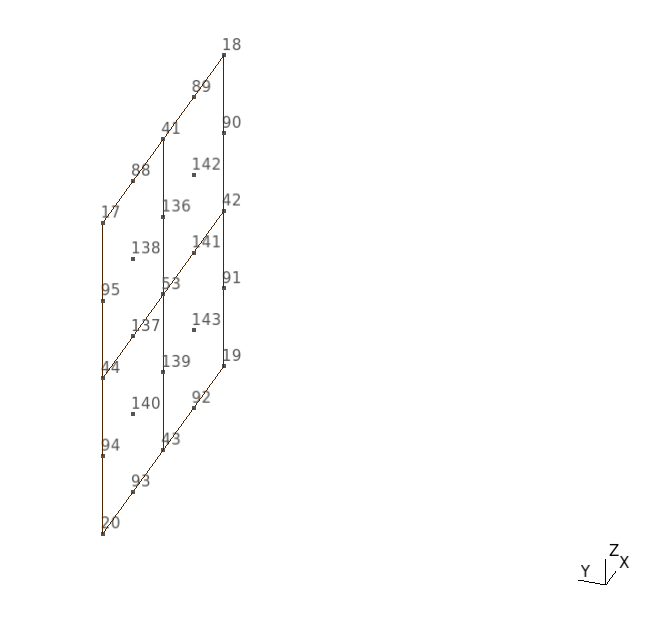
\includegraphics[width=\textwidth]{mesh_3.png}
    \caption{Left wall}
    \label{fig:g5}
  \end{subfigure}
  \hfill
  \begin{subfigure}[b]{0.48\textwidth}
    \centering
    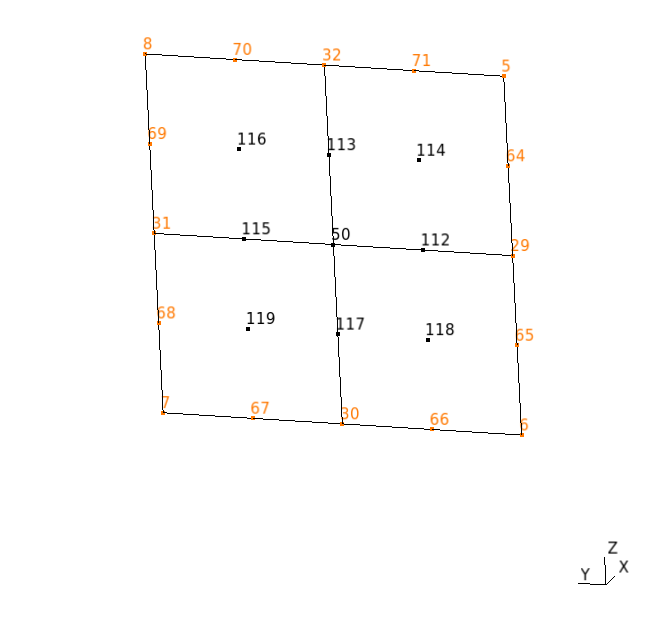
\includegraphics[width=\textwidth]{mesh_5.png}
    \caption{Back wall}
    \label{fig:g3}
  \end{subfigure}
  \hfill
  \begin{subfigure}[b]{0.48\textwidth}
    \centering
    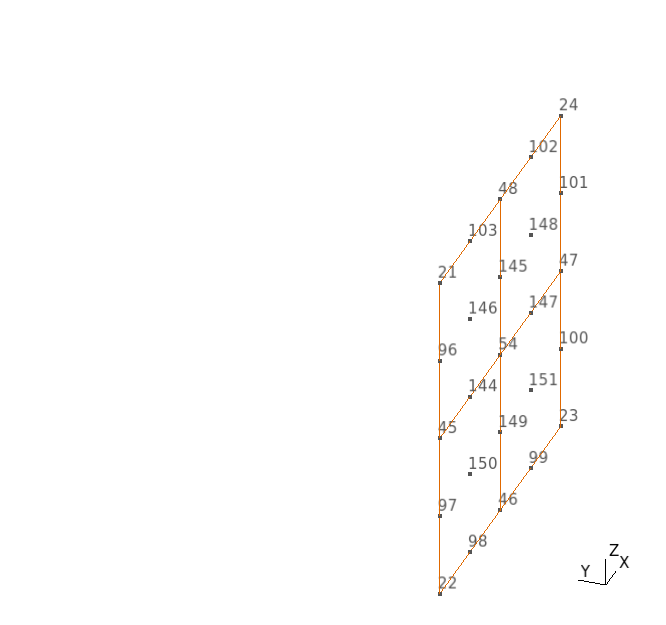
\includegraphics[width=\textwidth]{mesh_4.png}
    \caption{Right wall}
    \label{fig:g5}
  \end{subfigure}  
  \caption{Mesh. Note the multiple nodes along the boundary of each boundary piece.}
  \label{fig:geometry_partition}
\end{figure}

\subsection{Input data file}

The input data file contains data sections which defines the problem to be solved. The order of each data section is not important, but here we will follow a reasonably logical one.

The input data file begins with the definition of the type of problem (\texttt{[problem]} data section):
\begin{Verbatim}[frame=single, fontsize=\small, label=room.dat]
[problem]
type = mechanics
analysis = harmonic
n = 3D
\end{Verbatim}

Next, the frequencies to be analyzed are defined: 50 frequencies linearly distributed between 1 Hz and 300 Hz. This is done in the \texttt{[frequencies]} data section:
\begin{Verbatim}[frame=single, fontsize=\small, label=room.dat]
[frequencies]
Hz
lin
50
1.
300.000000
\end{Verbatim}

Then, the type of mesh format and the mesh file path are defined in the \texttt{[settings]} data section:
\begin{Verbatim}[frame=single, fontsize=\small, label=room.dat]
[settings]
mesh_file_mode = 2 "cube.msh"
\end{Verbatim}

Next, the list of boundary partitions are define in the data section \texttt{[boundaries]}.
\begin{Verbatim}[frame=single, fontsize=\small, label=room.dat]
[boundaries]
6
1 1 ordinary
2 2 ordinary
3 3 ordinary
4 4 ordinary
5 5 ordinary
6 6 ordinary
\end{Verbatim}
The data section starts by defining the number of boundaries, and then each boundary is specified in a separate line. Each boundary is defined by giving first the boundary identifier to be used within the solver, then the ``PhysicalName'' identifier which defines the mesh of the boundary, and finally the class of boundary, which may be \texttt{ordinary} or \texttt{crack-like}. In our case, they all are ordinary boundaries. Note that each boundary identifier does not need to be the same as the ``PhysicalName'' identifier, although it is certainly useful to do so in some problems. The only requisite for boundary identifiers is to be greater than 0.

\begin{figure}[h]
\centering
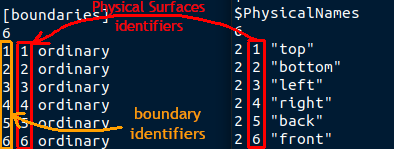
\includegraphics[scale=0.5]{boundaries_physical.png}
\caption{Left: input data file (\texttt{room.dat}). Right: Gmsh mesh file (\texttt{cube.msh}).}
\end{figure}

Now, the material properties are defined in the \texttt{[[materials]]} data section:
\begin{Verbatim}[frame=single, fontsize=\small, label=room.dat]
[materials]
1
1 fluid c 343. rho 1.25
\end{Verbatim}
The data section starts with a line defining the number of materials to be defined, and then the list of materials. In our case, we define the material with identifier 1 as a fluid with wave propagation speed of $c=343\,\mathrm{m/s}$, and density $\rho=1.25,\mathrm{kg/m^3}$, i.e. air.

Then, the list of subdomains (regions are called) can be defined in the \texttt{[regions]} data section. The first line again defines the number of regions (1 in this case). Then  a block of data is required for each region. Such block of data starts with the region identifier and the type of regions discretization (boundary elements in this case). The next line contains the list of boundary partitions which defines the boundary of the subdomain: in this case there are 6 boundaries with identifiers 1, 2, 3, 4, 5 and 6. These identifiers may have a negative sign, which indicates that that the orientation are reversed (this may be necessary when boundary orientation change is required at this stage). Next, the material is indicated by starting the line with the keyword \texttt{material} followed by the material identifier. The next two lines contains respectively the list of body loads and incident fields to be considered in this subdomain, both are zero in this case.
\begin{Verbatim}[frame=single, fontsize=\small, label=room.dat]
[regions]
1

1 be 
6 1 2 3 4 5 6
material 1
0
0
\end{Verbatim}

Finally, the boundary conditions are defined in the \texttt{[conditions over be boundaries]} data section. This data section requires the keyword \texttt{boundary} followed by the identifier and \texttt{:}, then an integer which must be 0 for prescribed pressure or 1 for prescribed normal displacement, and then the value of the boundary condition:
\begin{Verbatim}[frame=single, fontsize=\small, label=room.dat]
[conditions over be boundaries]
boundary 1: 1 (0.,0.)
boundary 2: 1 (0.,0.)
boundary 3: 1 (0.,0.)
boundary 4: 1 (0.,0.)
boundary 5: 0 (1.,0.)
boundary 6: 0 (0.,0.)
\end{Verbatim}

\section{Run}

Assuming that the mesh file has been generated, in order to run the solver you must execute (GNU/Linux terminal):
\begin{Verbatim}[frame=single, fontsize=\small, label=command line]
$ multifebe -i room.dat
\end{Verbatim}


\section{Post-processing}

In this simple example, we would like to simply verify that the obtained numerical result agrees with the analytical results. In order to do so, we have decided to compare the fluid displacement at $x=0$ m. 

The file \texttt{room.dat.nso} contains all the nodal results in a file format defined in the manual. In order to extract and plot the required result, we extract the nodal results of a given node (in our case node 1084 located at $(0,1.5,1.5)$ m) using the GNU/Linux tools \texttt{awk} and GNUPlot. See the attached \texttt{*.gp} file. You could do this also with a spreadsheet program by importing the file as a fixed width field table, and then filtering the rows.

Figure \ref{fig:sol} shows a comparison between the obtained numerical results against the analytical solution for the fluid displacement at $x=0$ m, where a very good agreement is obtained. 
 
% to be done: 
% - include internal point solutions
% - color map with pressures using gmsh
% - plot the pressure along x (numerical vs analytical)
 
\begin{figure}[h]
\centering
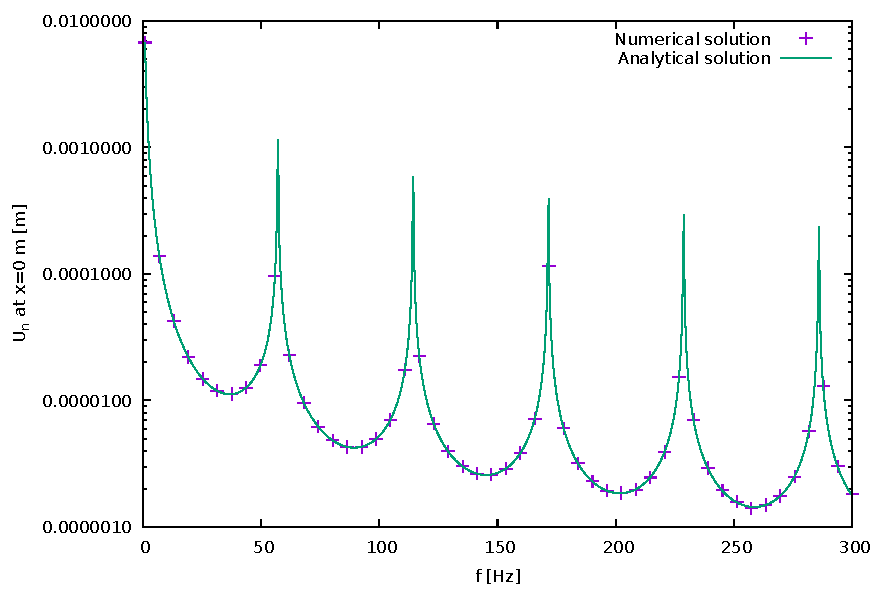
\includegraphics{solution1.pdf}
\caption{Fluid normal displacement at $x=0$ m (front wall).}
\label{fig:sol}
\end{figure}

\begin{thebibliography}{99}
	\bibitem{gmsh} C. Geuzaine and J.-F. Remacle, ``Gmsh: a three-dimensional finite element mesh generator with built-in pre- and post-processing facilities." \textit{International Journal for Numerical Methods in Engineering}, Volume 79, Issue 11, pages 1309--1331, (2009)
	
	\bibitem{gmshweb} C. Geuzaine and J.-F. Remacle, ``Gmsh." \url{http://gmsh.info/}
	
	\bibitem{dominguez} J. Domínguez. Boundary Elements in Dynamics. WIT Press. 1993.
	
	\bibitem{maeso} O. Maeso and J.J. Aznárez. Estrategias para la reducción del impacto acústico en el entorno de carreteras: una aplicación del método de los elementos de contorno. Universidad de Las Palmas de Gran Canaria. 2005.

	\bibitem{brebbia} C. Brebbia and J. Domínguez. Boundary Elements: an introductory course. WIT Press. 1984.
	
\end{thebibliography}

\end{document}
